In this section we evaluate the capacity of the AWP algorithm and the ADT procedure to accelerate DNNs training. 
We show how our proposals are able to accelerate the training phase of relevant DNN models without reducing the accuracy of the network. 

\subsection{Methodology}
\label{sec:evaluation1}

\begin{figure*}[!bhtp]
    \hbox{%\hspace{7.0mm}
        \centerline{
            \includegraphics[scale=0.450]{bitpack/figs/vgg/small_3/vgg_validation_top5_64-$A^2$DtWp.pdf}
            \includegraphics[scale=0.450]{bitpack/figs/vgg/small_3/vgg_validation_top5_32-$A^2$DtWp.pdf}
        }
    }
    \hbox{%\hspace{7.0mm}
        \centerline{
            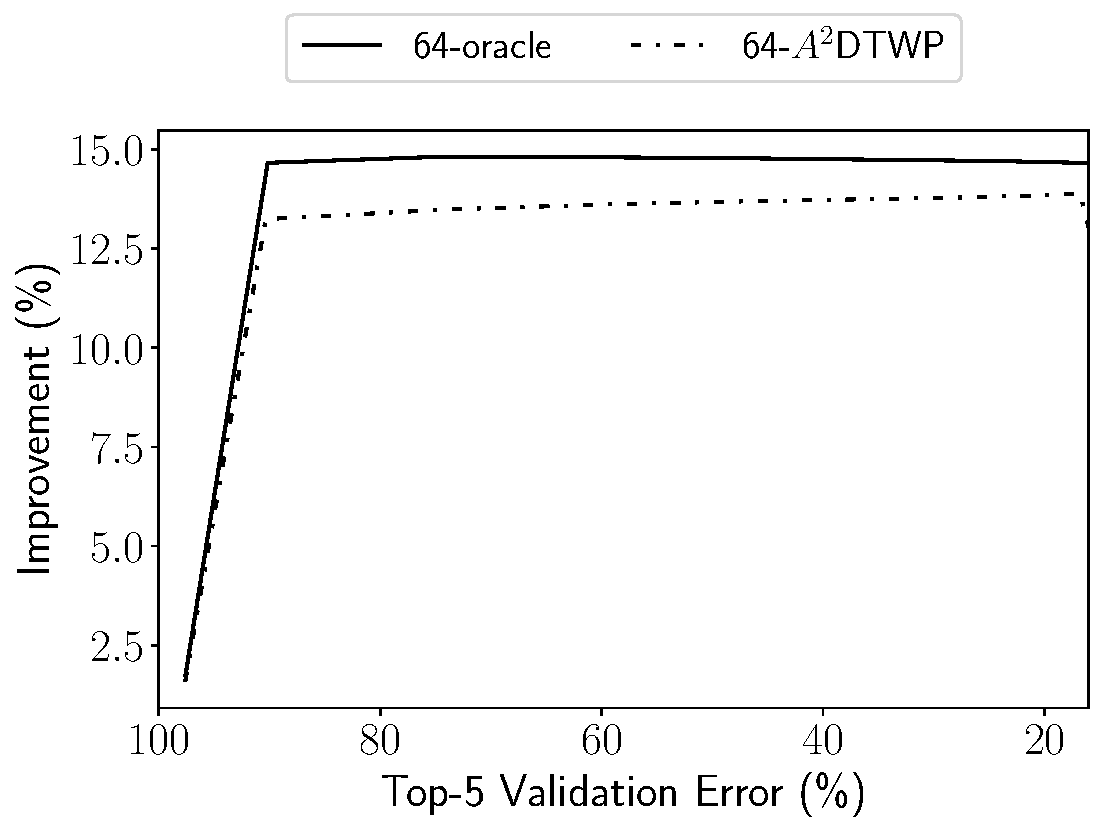
\includegraphics[scale=0.450]{bitpack/figs/vgg/small_3/vgg_train_improvement_agg_top5_64-baseline.pdf}
            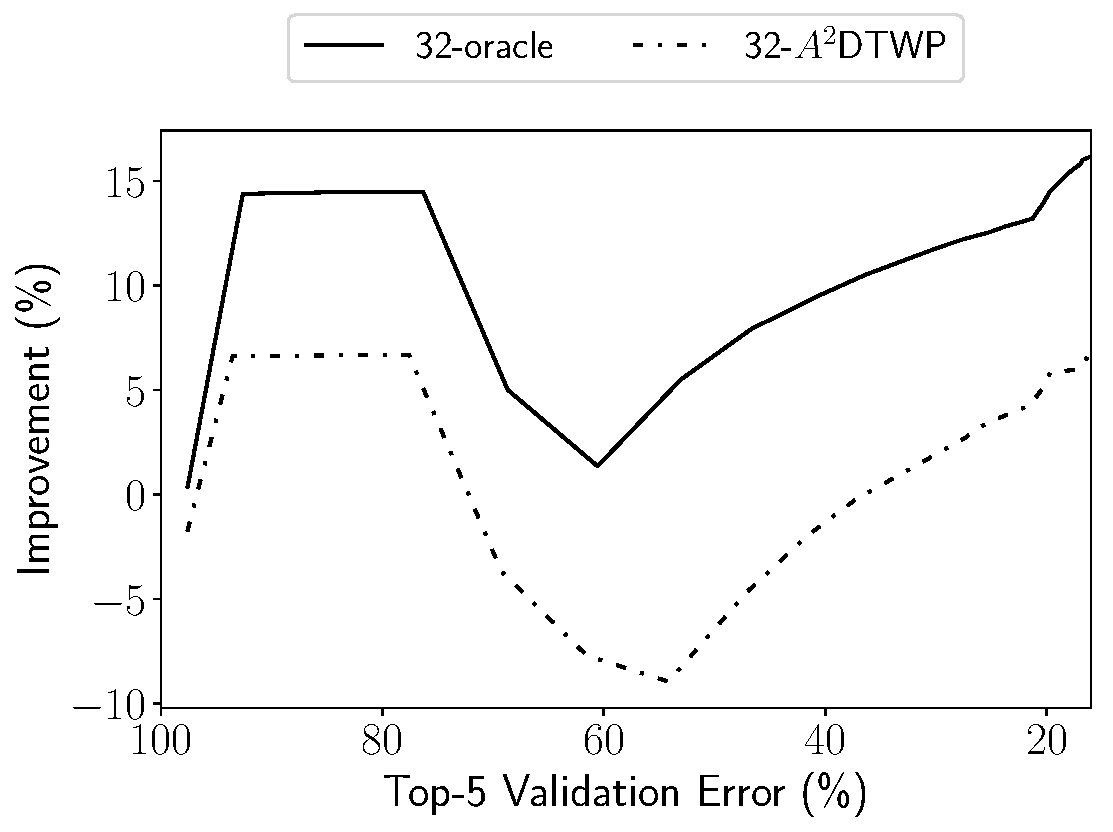
\includegraphics[scale=0.450]{bitpack/figs/vgg/small_3/vgg_train_improvement_agg_top5_32-baseline.pdf}
        }
    }
    \caption{VGG training considering 64 and 32 batch sizes. The 
    two upper plots show the top-5 validation error evolution of
    \textit{baseline}, \textit{oracle} and \textit{$A^2$DTWP}.
    The two bottom figures provide information on the performance improvement of
    \textit{oracle} and \textit{$A^2$DTWP} against \textit{baseline} during the
    training process. Experiments run on the x86 system.
    %\rephrased{Figures upgraded from using continuous lines to using points}
    }
    \label{vgg_improv}
    %\vspace{-0.5cm}
\end{figure*}

%We conduct a set of experiments on several batch sizes (16, 32, 64) for both Alexnet and VGG. 
Our experimental campaign considers batch sizes of 64, 32 and 16 for the Alexnet and VGG models and 128, 64 and 32 for the Resnet network.
For each model and batch size, the \emph{baseline} run uses the 32-bit Floating Point precision for the whole training. 
The data represention formats we consider to transfer weights from the CPU to the GPU are:
8-bit (1 bit for sign, 7 bits for exponent), 16-bit (1 bit for sign, 8 for exponent, 7 for mantissa), 24-bit (1 bit for sign, 8-bits for exponent and 15 bits for mantissa) and 32-bits (1 bit for sign, 8 bits for exponent and 23 bits for mantissa).
We train the network models with dynamic data representation by applying the AWP algorithm along with the ADT procedure.
We denote this approach combining ADT and AWP as \textit{$A^2$DTWP}.  
For each DNN and batch size, we select the data representation format that first 
reaches the 35\%, 25\% and 15\% accuracy thresholds for Resnet, Alexnet and VGG, respectively, and we 
denote this approach as \emph{oracle}.
For the case of the \emph{oracle} approach, data compression is done via ADT.
The closer \textit{$A^2$DTWP} is to \emph{oracle}, the better is the AWP algorithm in identifying the best data representation format.

During training we sample data in terms of elapse time and validation error every 4000 batches. 
The total number of training batches corresponding to the whole ImageNet200 dataset are 16020, 8010, 4005 and 2002 for batch sizes 16, 32, 64 and 128, respectively.
The values of $AWP$ parameters $T$, $INTERVAL$, and $N$ are determined in the following way:
In the case of $T$ we monitor the execution of several epochs until we observe a drop in the validation error. 
We then measure the average change, considering all layers, of weights' $l^2$-norm during this short monitoring period.
The obtained values of $T$ are $-5\times10^{-2}$, $-2\times10^{-3}$ and $-2\times10^{-5}$ for Alexnet, VGG and Resnet, respectively.
We set the $INTERVAL$ parameter to $4000$ for both AlexNet and VGG and $2000$ for Resnet. 
These values correspond to a single batch (for the ImageNet200 dataset and batch sizes 64 and 128) and avoid premature precision switching due to numerical fluctuations.  
We set $N$ to $8$ since the smallest granularity of our approach is 1 byte.
AWP initially applies 8-bit precision to all layers.
We use ImageNet200 in Sections~\ref{sec:alexnet}, ~\ref{sec:VGG}, ~\ref{sec:Resnet}, ~\ref{sec:Average}, and ~\ref{sec:performance}.
Section~\ref{sec:ImageNet1000} uses ImageNet1000.

\subsection{Evaluation on Alexnet}
\label{sec:alexnet}
The evaluation considering the Alexnet model on the x86 system is shown in  
Figure~\ref{alex_improv}, which plots detailed results considering batch sizes of 
32 and 16, and Figure~\ref{fig:all}, which shows the total execution time of the 
\textit{oracle} and \textit{$A^2$DTWP} policies normalized to the \textit{baseline} 
for the 64, 32 and 16 batch sizes on both the x86 and the POWER systems.
The two top plots of Figure~\ref{alex_improv} depict how the validation error of the 
\textit{baseline}, \textit{oracle}, and \textit{$A^2$DTWP} policies evolves 
over time for the 32 and the 16 batch sizes until the 25\% accuracy is reached.
The two bottom plots provide information regarding the performance 
improvement of both \textit{oracle} and \textit{$A^2$DTWP} over the 
32-bit \textit{baseline} with regard to a certain validation error. 
Such performance improvement is computed by looking at the time required by the 
\textit{oracle} and \textit{$A^2$DTWP} techniques to reach a certain validation error with respect to the \textit{baseline}.

It can be observed in the upper left-hand side plot of Figure~\ref{alex_improv} how 
the \textit{oracle} and the \textit{$A^2$DTWP} approaches are 10.82\% and 6.61\% faster than the baseline, respectively, to reach the 25\% top-5 validation error when using a 32 batch size.
The upper right-hand side plot shows results considering a 16 batch size. 
The improvements achieved by the 
\textit{oracle} and \textit{$A^2$DTWP} approaches are 11.52\% and 10.66\%, respectively.
This demonstrates 
the efficiency of the ADT procedure in compressing and decompressing the network weights without undermining the performance benefits obtained from sending less data
from the CPU device to the GPU.
It also demonstrates the capacity of AWP to quickly identify the best data representation format per layer.

The two bottom plots of Figure~\ref{alex_improv} provide information on 
performance improvement of \textit{oracle} and \textit{$A^2$DTWP} over the \textit{baseline} during the training process.
%One of the right-hand side plots of Figure~\ref{alex_improv} shows results when considering the 32 batch size.
For the 32 batch size, \textit{oracle} reaches a peak improvement of 24.11\% when the 90\%  
validation error is reached and steadily declines from that point although it keeps a significant 
improvement of 10.82\% over the \textit{baseline} once the 25\% top-5 validation error is reached. 
\textit{$A^2$DTWP} falls in-between the \textit{baseline} and the \textit{oracle}  
and keeps its improvement above 7.03\% until it reaches the 27\% top-5 validation error.
Once it reaches the 25\% validation error \textit{$A^2$DTWP} is 6.51\% faster than the \textit{baseline}.
In conclusion, the \textit{$A^2$DTWP} policy is able to provide performance 
improvements that are close to the ones achieved by the best possible accuracy.
%while the \textit{best} reaches 9.39\% at 25\% validation error.
For the 16 batch size, the performance benefits of the 
\textit{oracle} policy reach a 41.64\% peak at the 94\% validation error point.
The \textit{$A^2$DTWP} policy reaches its maximum performance benefit, 34.21\%, when the validation error is 97\%.
At the 25\% validation error point, the \textit{oracle} and the 
\textit{$A^2$DTWP} policies reach 13.00\% and 10.75\% performance improvement, respectively.
Overall, results considering the Alexnet network for batch sizes 
32 and 16 confirm that \textit{$A^2$DTWP}, which combines both the 
AWP algorithm and the ADT procedure, successfully delivers very similar 
performance benefits to the best possible accuracy.

Figure~\ref{fig:all} shows the normalized execution time of the \textit{oracle} 
and \textit{$A^2$DTWP} policies with respect to the 32-bit FP \textit{baseline} on the x86 and the POWER systems. 
The top chart reports performance improvements of 10.75\%, 6.51\%, and 0.59\% for batch sizes 16, 32 and 64 in
the case of Alexnet runnig on the x86 system.  
For the 64 batch size, the marginal gains of \textit{$A^2$DTWP} over the \textit{baseline} are due the poor performance of the 8-bits format employed by \textit{$A^2$DTWP} at the beginning of the training process.
This format does not contribute to reduce the validation error for the 64 batch case, which makes the \textit{$A^2$DTWP} policy to fall behind the \textit{baseline} at the very beginning of the training process.  
Although \textit{$A^2$DTWP} eventually increases its accuracy and surpases the \textit{baseline}, it does not provide the same significant performance gains for Alexnet as the ones observed for batch sizes 16 and 32.

\textit{$A^2$DTWP} performance improvements on the POWER system in the case of 
Alexnet are 18.61\%, 14.25\% and 10.01\% with respect to the \textit{baseline} for batch sizes 16, 32 and 64, respectively.  
The POWER system achieves larger performance improvements than x86 since the 
Bitpack procedure can be further parallelized over the 40 cores of the POWER9 
multicore chips than the 16 cores available in the Haswell multicore devices of the x86 system. 
This mitigates the costs of weigths' compression and thus provides larger performance improvements. 

\subsection{Evaluation on VGG}
\label{sec:VGG}

Figure~\ref{vgg_improv} shows results for batch sizes 64 and 32 when using the 
VGG architecture on the x86 system. 
The upper figures display the temporal evolution of the validation error until the 15\% top-5 validation error is reached.
Like in Alexnet, both the \textit{$A^2$DTWP} and the \textit{oracle} policies outperform the \textit{baseline}.
In the case of batch size 64, both \textit{oracle} and \textit{$A^2$DTWP} 
display a similar evolution in terms of validation error, which translates to 
very close performance improvement over the baseline. 
They maintain an overall improvement of over 13.00\% against the \textit{baseline} 
during most of their training. The \textit{$A^2$DTWP} technique outperforms the baseline by 
12.88\% when reaches 15\% of top-5 validation error while the 
\textit{oracle} policy achieves the same improvement.
For batch size 32 the final improvement achieved by \textit{$A^2$DTWP} over the baseline is 5.02\%.
This improvement is not as large as the one achived for the 64 batch size since the AWP algorithm does not identify a numerical precision able to beat the \textit{baseline} until the 57\% validation error is reached, as it can be seen in the bottom right hand side plot of Figure~\ref{vgg_improv}. 
%Despite this issue, \textit{$A^2$DTWP} still achieves a remarkable performance improvement of {\bf XX\%} over the baseline.

Figure~\ref{fig:all} shows the normalized execution time of \textit{$A^2$DTWP} 
and \textit{oracle} with respect to the \textit{baseline} for VGG considering 
batch sizes of 16, 32 and 64 on the x86 and POWER systems.
When applied to the VGG model on the x86 system, \textit{$A^2$DTWP} outperforms the 32-bit Floating Point \textit{baseline} by 12.88\%, 5.02\% and 7.31\% for batch sizes 64, 32 and 16, respectively.
Despite the already described issues suffered by the \textit{$A^2$DTWP} technique when applied to the 32 batch size, this approach achieves very remarkable performance improvements over the baseline in all considered scenarios. 

The performance improvements observed when trying VGG on the POWER system are even higher.
\textit{$A^2$DTWP} outperforms the \textit{baseline} by 28.21\%, 20.19\% and 11.13\% when using the 16, 32 and 64 batch sizes, respectively.
The performance improvement achieved on the POWER system are larger than the ones observed for x86 since the Bitpack procedure can be parallelized over 40 cores when running on the POWER system.
We observe the same behavior for Alexnet, as Section~\ref{sec:alexnet} indicates.

\subsection{Evaluation on Resnet}
\label{sec:Resnet}
We display the normalized execution time of the \textit{$A^2$DTWP} and the \textit{oracle} policies when applied to the Resnet model using batch sizes of 128, 64 and 32 in Figure~\ref{fig:all}.
In the case of Resnet we do not show detailed plots describing the evolution of 
the validation error during training because its behavior is very close to some previously displayed scenarios like VGG.
On the x86 system, \textit{$A^2$DTWP} beats the 32-bit Floating Point baseline by 4.94\%, 4.39\% and 3.11\% for batch sizes of 128, 64 and 32, respectively, once a top-5 validation error of 30\% is reached.
The relatively low performance improvement achieved in the case of 32 batch size is due to a late identification of a competitive numerical precision, as it happens in the case of VGG and batch size 32.

The performance gains on the POWER system display a similar trend as the ones achieved on x86. 
While they show the same low improvement for the 32 batch size, 2.12\%, \textit{$A^2$DTWP} achieves 6.92\% and 11.54\% performance gains for batch sizes 64 and 128, respectively.
\textit{$A^2$DTWP} achieves the largest performance improvement with respect to the 32-bit \textit{baseline} when run on the POWER system due to the reasons described in Sections~\ref{sec:alexnet} and~\ref{sec:VGG}.

\subsection{Average Performance Improvement}
\label{sec:Average}
The average performance improvement of \textit{$A^2$DTWP} over the 
\textit{baseline} considering the Alexnet, VGG and Resnet models reach 6.18\% and 11.91\% on the x86 and the POWER systems, respectively. 
As we explain in previous sections, \textit{$A^2$DTWP} obtains larger improvements on the POWER system than on  
x86 since the ADT procedure can be further parallelized over the 40 cores of the POWER9 multicore devices.
In contrast, the two Haswell devices of the x86 system offer just 16 cores for ADT.

The combination of the AWP algorithm and the ADT procedure properly adapts the precision of each network layer and compresses the corresponding weigths with a minimal overhead.
The large performance improvement obtained while training deep networks on two high-end computing systems demonstrate the effectiveness of \textit{$A^2$DTWP}.

\begin{figure*}%[!bhtp]
    \centerline{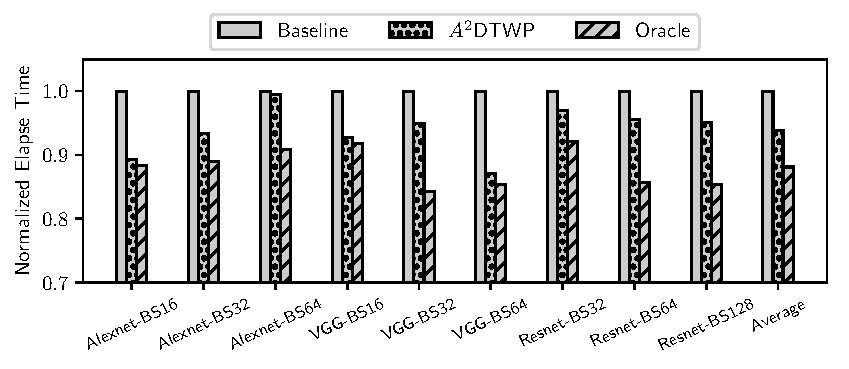
\includegraphics[scale=0.85]{bitpack/figs/all_bars.pdf}}
    %\vspace{-0.2cm}
    \centerline{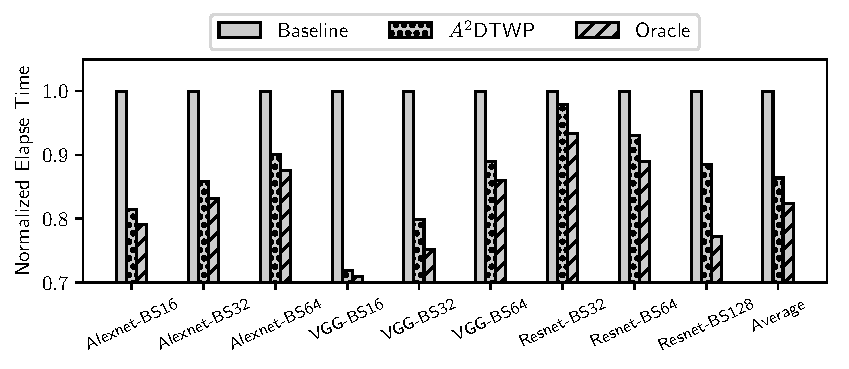
\includegraphics[scale=0.85]{bitpack/figs/all_bars_p9.pdf}}
    %\vspace{-0.5cm}
    \caption{Normalized execution times of the \textit{$A^2$DTWP} and the \textit{oracle} policies with respect to the baseline. 
Results obtained on the x86 system appear in the upper plot while the evalution on the POWER system appears at the bottom.} 
    \label{fig:all}
\end{figure*}

\subsection{$A^2DTWP$ Performance Profile}
\label{sec:performance}
This section provides a detailed performance profile describing the effects of 
applying $A^2DTWP$ when training the VGG network model with batch size 64 on the x86 and POWER systems described in section~\ref{sec:platform}.
To highlight these effects we also show a performance profile of applying 32-bit 
Floating Point format during training.
The main kernels involved in the training process and their corresponding average execution time in milliseconds are shown in Tables ~\ref{table:performance} and~\ref{table:performance_p9}.
Each kernel can be invoked multiple times by different network layers and it can be overlapped with other operations while processing a batch.
Tables~\ref{table:performance} and~\ref{table:performance_p9} display for all kernels the average execution time of their occurrences within a batch when run on the x96 and the POWER systems, respectively.

Results appearing in Table~\ref{table:performance} show how time spent transferring 
data from the CPU to the GPU accelerators when applying $A^2DTWP$ on the x86 system, 52.27 ms, 
is significantly smaller than the cost of performing the same operation when using the 32-bit configuration, 153.93 ms. 
This constitutes a 2.94x execution time reduction that compensates the cost of the operations involved in the ADT routine, Bitpack and
Bitunpack, and in the AWP algorithm, the $l^2$-norm computation.
On POWER we observe a similar reduction of 3.20x in the time spent transferring
data from the CPU to the GPUs when applying $A^2DTWP$.
These reductions in terms of CPU to GPU data transfer time are due to a close to 3x reduction in terms of weights size enabled by $A^2DTWP$.
The average execution time of operations where the $A^2DTWP$ technique plays no role remains very similar for the 32-bit Floating Point baseline and $A^2DTWP$ in both systems, as expected.
Tables~\ref{table:performance} and~\ref{table:performance_p9} indicate that performance gains achieved by $A^2DTWP$ are due to data motion reductions, which validates the usefulness of $A^2DTWP$.

Tables~\ref{table:performance} and~\ref{table:performance_p9} also display the overhead associated with AWP and ADT in terms of milliseconds.
The AWP algorithm spends most of its runtime computing the $l^2$-norm of the weights, which takes a total of 3.88 ms within a batch on the x86 system. 
On POWER, the cost of computing the $l^2$-norm of the weights is 0.93 ms.
The other operations carried out by AWP have a negligible overhead.
The two fundamental procedures of ADT are the Bitpack and Bitunpack routines, which take 19.71 and 4.51 ms to run within a single batch on the x86 system.
For the case of POWER, Bitpack and Bitunpack take 10.51 and 1.11 ms, respectively.
Overall, measurements displayed at Table~\ref{table:performance} indicate that AWP and ADT constitute 1.05\% and 6.60\% of the total batch execution time, respectively, on x86.
On the POWER system, AWP and ADT constitute 0.54\% and 6.82\% of the total batch execution time according to Table~\ref{table:performance_p9}. 
Figures ~\ref{alex_improv}, ~\ref{vgg_improv} and ~\ref{fig:all} account for this overhead in the results they display.

\begin{table}
    \caption{Performance profiles of both the $A^2DTWP$ and the 32-bit Floating 
    Point approaches expressed in milliseconds on the x86 system. 
    We consider the VGG network model with batch size 64.} 
    %\vspace{-0.35cm}
    \centering
    \begin{tabular}{|P{4.5cm}|P{2.5cm}|P{2.5cm}|}
    \hline
    %\rowcolor{LightCyan}
    & \textbf{32-bit FP} & $\mathbf{A^2DTWP}$\\
    \hline
    %\rowcolor{LightCyan}
    Data Transfer CPU$\rightarrow$GPU& 153.93 & 52.27 \\
    \hline
    %\rowcolor{LightCyan}
    Data Transfer GPU$\rightarrow$CPU& 68.51 & 73.55 \\
    \hline
    %\rowcolor{LightCyan}
    Convolution & 128.72 & 126.13\\
    \hline
    %\rowcolor{LightCyan}
    Fully-connected & 33.51 & 34.17 \\
    \hline
    %\rowcolor{LightCyan}
    Gradient update & 54.39 & 52.86\\
    \hline
    %\rowcolor{LightCyan}
    AWP ($l^2$-norm) & N/A & 3.88 \\
    \hline
    %\rowcolor{LightCyan}
    ADT (Bitpack) & N/A & 19.71 \\
    \hline
    %\rowcolor{LightCyan}
    ADT (Bitunpack) & N/A & 4.51 \\
    \hline
    \end{tabular}
    \label{table:performance}
\end{table}

\begin{table}
    \caption{Performance profiles of both the $A^2DTWP$ and the 32-bit Floating 
    Point approaches expressed in milliseconds on the POWER system. 
    We consider the VGG network model with batch size 64.} 
    %\vspace{-0.35cm}
    \centering
    \begin{tabular}{|P{4.5cm}|P{2.5cm}|P{2.5cm}|}
    \hline
    & \textbf{32-bit FP} & $\mathbf{A^2DTWP}$ \\
    \hline
    Data Transfer CPU$\rightarrow$GPU& 39.12 & 12.21 \\
    \hline
    Data Transfer GPU$\rightarrow$CPU& 17.34 & 17.87 \\
    \hline
    Convolution & 69.78 & 71.21\\
    \hline
    Fully-connected & 12.66 & 13.51 \\
    \hline
    Gradient update & 41.29 & 42.98\\
    \hline
    AWP ($l^2$-norm) & N/A & 0.93 \\
    \hline
    ADT (Bitpack) & N/A & 10.51 \\
    \hline
    ADT (Bitunpack) & N/A & 1.11 \\
    \hline
    \end{tabular}
    \label{table:performance_p9}
\end{table}

\subsection{Experiments with ImageNet1000}
\label{sec:ImageNet1000}
We run experiments considering ImageNet1000 to confirm they display the same trends as executions with ImageNet200. 
Network parameters are the same as the ones described in Section~\ref{sec:setup}.
$AWP$ parameters are the ones described in Section~\ref{sec:evaluation1}.
The experimental setup of the evaluation considering ImageNet1000 is the same as the one we use for ImageNet200.
We consider batch sizes that produce the fastest 32-bit FP training for each one of the network models: 64, 64, and 128 for Alexnet, VGG and Resnet, respectively.


Figure~\ref{fig:ImageNet1000} displays results corresponding to the experimental campaign with ImageNet1000 on the x86 system.
In the x-axis we display different epoch counts for each one of the three models: 4, 8, 12, 16, and 20 epochs for Alexnet; 2, 4, 6, and 8 for VGG; and 4, 8, 12, and 16 epochs for Resnet.
The y-axis displays the normalized elapsed time of \textit{$A^2$DTWP} with respect to the the 32-bit Floating Point \textit{baseline} per each model and epoch count.
For the case of Alexnet with batch size 64, \textit{$A^2$DTWP} is slightly faster than the \textit{baseline} as it displays a normalized execution time of 0.995, 0.992, 0.992, 0.996, and 0.990 after 4, 8, 12, 16 and 20 epochs, respectively.
Figure~\ref{fig:all} also reports small gains for the case of Alexnet with batch size 64, which confirms that experiments with ImageNet1000 show very similar trends as the evaluation with ImageNet200.
When applying \textit{$A^2$DTWP} to VGG with 64 batch size, it displays a normalized execution time of 0.907, 0.920, 0.936, and 0.932 with respect to the \textit{baseline} after running 2, 4, 6 and 8 training epochs, respectively.
For the Resnet example, we observe normalized execution times of 0.765, 0.770, 0.778, and 0.777 for \textit{$A^2$DTWP} after 4, 8, 12, and 16 training epochs, respectively,
which constitutes a significant performance improvement.

\begin{figure}%[!bhtp]
    \centerline{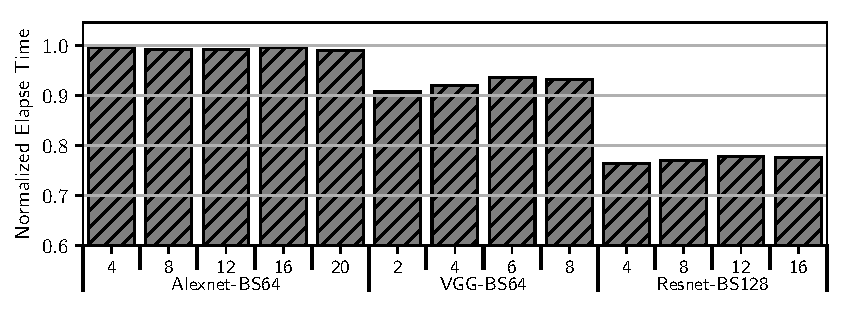
\includegraphics[scale=0.85]{bitpack/figs/imagenet-1k-3net.pdf}}
    \caption{Normalized execution time of \textit{$A^2$DTWP} with respect to \textit{baseline} considering the Imagenet1000 data set. Training for Alexnet, VGG and Resnet considers up to 20, 8, and 16 epochs, respectively.}
    \label{fig:ImageNet1000}
\end{figure}

In terms of validation error, both \textit{$A^2$DTWP} and \textit{baseline} display very similar top-5 values at the end of each epoch.
For example, for the case of VGG, the Floating Point 32-bit \textit{baseline} approach displays a validation error of 88.04\% after 2 training epochs while \textit{$A^2$DTWP} achieves a validation error of 89.97\% for the same epoch count, that is, an absolute difference of 1.93\%.
After 4, 6, and 8 training epochs absolute distances of top-5 validation errors between \textit{$A^2$DTWP} and \textit{baseline} are 3.09\%, 0.47\%, and 0.71\%, respectively.
Top-5 validation error keeps decreasing in an analogous way for both \textit{baseline} and \textit{$A^2$DTWP} as training goes over more epochs, although \textit{$A^2$DTWP} is significantly faster.
Our evaluation indicates that \textit{$A^2$DTWP} can effectively accelerate training while achieving the same validation error as the 32-bit FP \textit{baseline} when considering ImageNet1000.
